\chapter{The ICE Model}
Several vertebrates, e.g. lizards, frogs, alligators and many birds, possess a hearing mechanism very different to
that of mammals: their tympanic membranes are coupled through large eustachian tubes and a large mouth cavity resulting in the influence of the vibrations of one tympanic membrane
on those of the other. This is illustrated in \ref{geckohead}. The typically small head sizes (compared to sound wavelength) of these animals result in
small phase differences (ITDs) and negligible amplitude difference (ILDs) between the ears. The coupling serves to enhance the ITDs and create ILDs
between the tympanal vibrations. These differences show directionality and serve as hearing cues for localization.

\begin{figure}[ht]
 \centering
 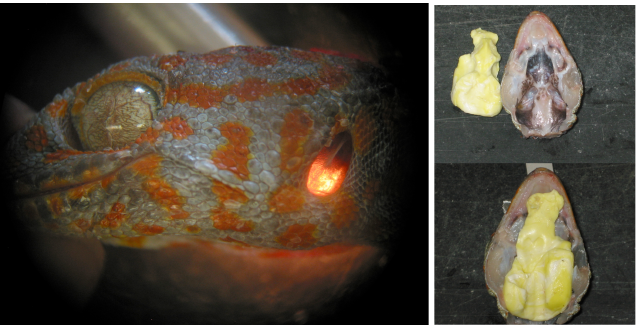
\includegraphics[width=.85\linewidth]{Diagrams/geckohead1.png}
 \caption[Illustration of a gecko's head]{Left: Picture of a Tokay gecko's head with the snout pointing to the left. The tympanic membrane is illuminated from behind by
 a light source on the other side of the head. The cartileginous extracolumella can be seen attached to the upper part of the membrane.
 Right: Cast imprint of the mouth cavity of the gecko with the snout pointing to the top. The figures illustrate the coupling of the tympani through the mouth cavity.
 Photographs courtesy of Jakob Christensen-Dalsgaard.}
  \label{geckohead}
\end{figure}

In this chapter we present a model for the
middle-ear of lizards - specifically the Tokay Gecko and the Common House Gecko. Our goal is to do this in the simplest possible way while ensuring an accurate reproduction of its main properties. 
The main components of such a 
system are the mouth-cavity, the two tympani and the two extracolumellar
footplates (one on each tympanum). In general, the shape of the mouth-cavity is highly irregular and therefore
not conducive to an analytical treatment. Moreover, the system corresponds to a pair of coupled second-order PDE's with
moving boundaries. For this reason we will need to make further approximations for the sake of expediency.

In order to make the system more analytically tractable we will, as before, study a geometry in which a pair of sectoral
membranes are coupled through a cylindrical cavity. The cylindrical geometry allows an accurately calculation of the 
pressure distribution inside the cavity at both low and high frequencies. By accounting for the presence of the asymetrically attached
extracolumella, we will also explain the complex vibration patterns of the membrane. At the end of this chapter, we will
have the main objects - the internal time differences (iTDs) and internal level differences (iLDs) - which 
quantify the response of the system as a function direction and frequency.

\section{Description}
In the earlier treatment of the ICE model, the mouth canal is modelled as a simple cylinder closed at 
both ends by rigidly clamped (baffled) circular membranes; these model the tympanic membranes. As shown 
in \cite{vossenthesis} and \cite{vossenjasa}, the length of the cylinder was chosen to be equal to the interaural distance and the radius of the model tympanum is
determined from the typical area of the realistic tympanum. The advantage of using a cylindrical cavity model for the mouth cavity is that the pressure
distribution inside the cavity is easy to calculate. The pressure distribution inside the cavity becomes highly non-uniform 
with increasing frequency and a cylindrical cavity simplifies its calculation. 

On the other hand, in this description the small area of the tympani results in a cavity volume which 
is an order of magnitude smaller than that of the realistic mouth-cavity in the corresponding animal. In general, a smaller volume results in a stronger coupling - both in terms of an increased iTD and an increased
iLD. For this reason, the earlier model overestimates the iTDs and iLDs at
low and high frequencies respectively.

In order to get around this problem we make some slight modifications to the model. We basically maintain the cylindrical shape of the internal 
cavity but require it to have a volume which is equal to that of the realistic cavity. We maintain the same tympanum size and interaural distance
and can therefore calculate the radius of the cylinder as,
\begin{align}
 a_{cyl}=\sqrt{\frac{V_{cav}}{\pi L}}
\end{align}
\begin{figure}[ht]
\begin{center}
\begin{subfigure}{1.0\textwidth}
 \centering
  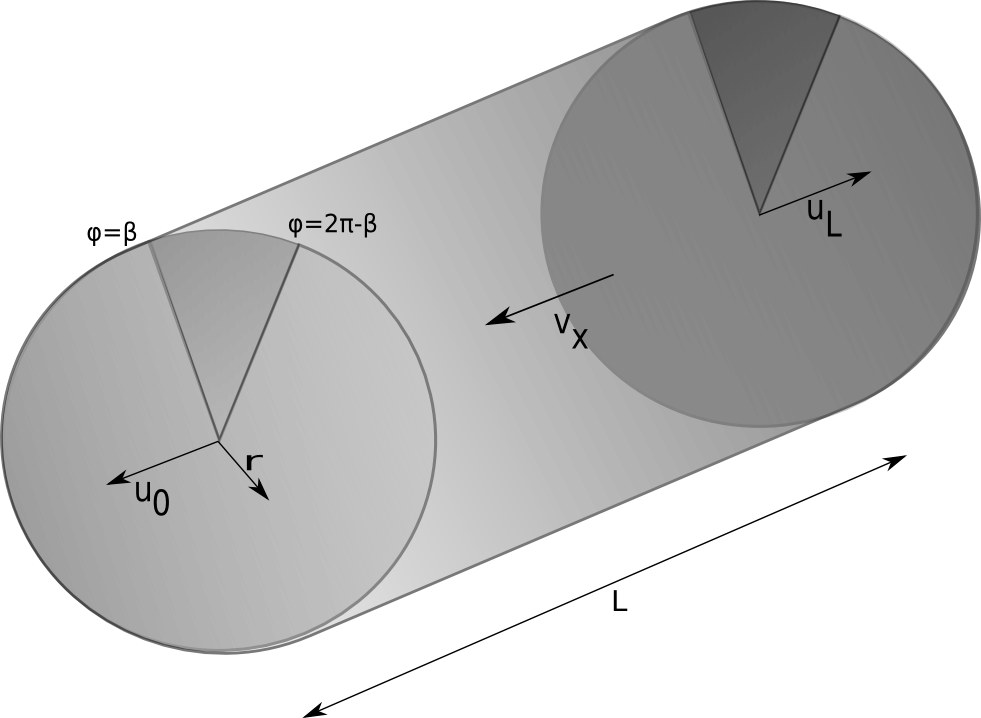
\includegraphics[width=.5\linewidth]{Diagrams/oldCylinder.png}
   \caption[Previous ICE Model Cylinder]{The previous geometric reprentation of the ICE model.}
  \label{oldICE}
\end{subfigure}

\begin{subfigure}{1.0\textwidth}
\centering
  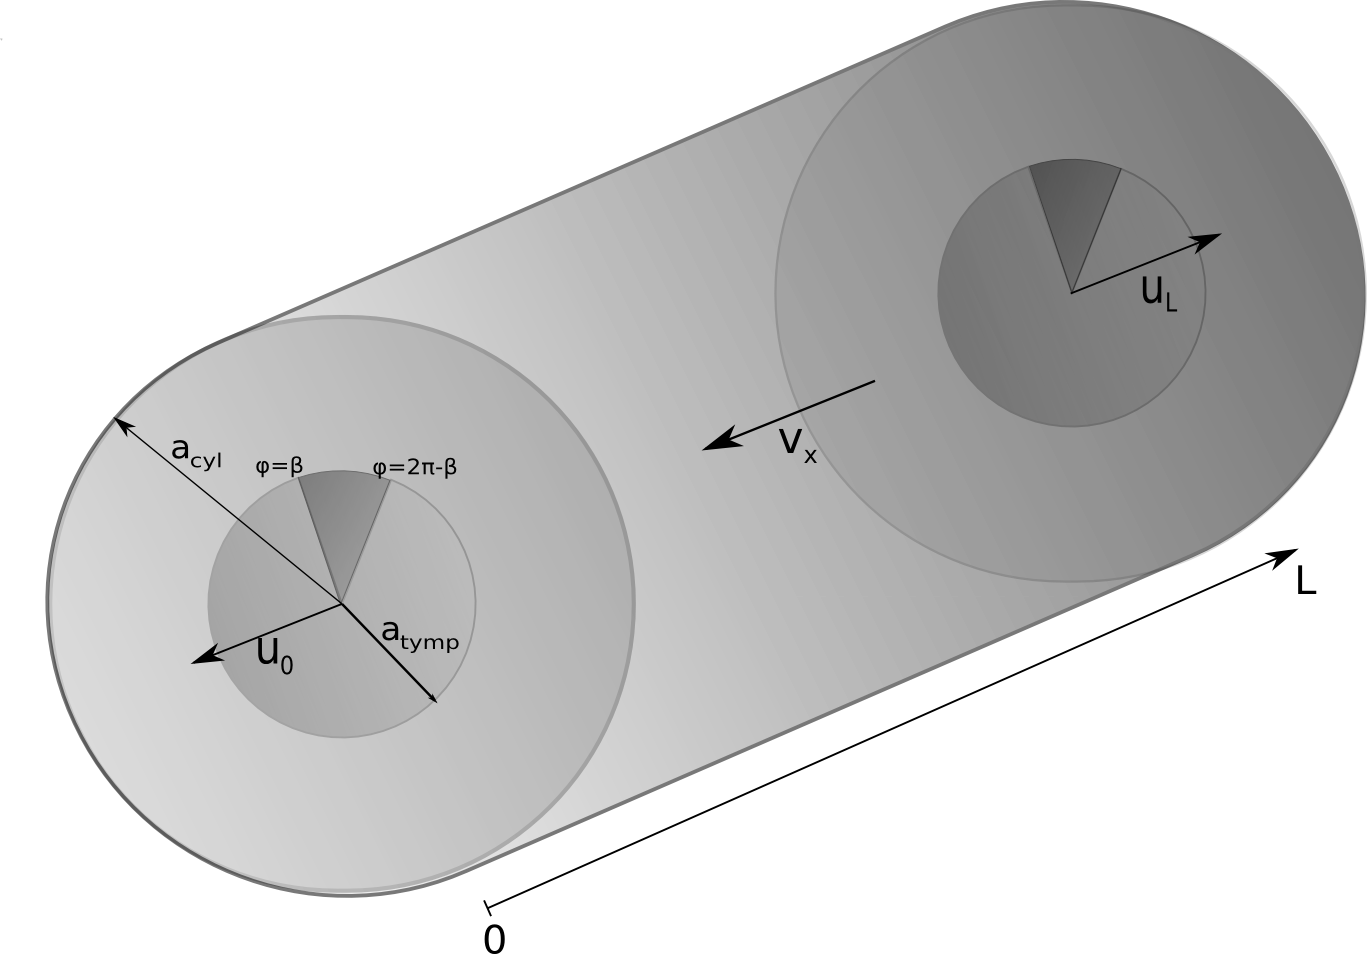
\includegraphics[width=.5\linewidth]{Diagrams/newCylinder.png}
  \caption[New ICE Model Cylinder]{The representation of the new model.}
  \label{newICE}
  \end{subfigure}
  \caption[Previous and current ICE model representations]{The bold arrows represent the direction conventions
  along the cylinder's axis. The new model is represented by a cylinder of radius $a_{cyl}$ and length $L$ closed
  at both ends by sectoral membrane of radius $a_{tymp}$.
  The darkly shaded region corresponds to the extracolumella (described in \ref{middleear}).}
\end{center}
\end{figure}
where $a_{cyl}$ is the cylinder radius and $L$ is the interaural distance. Simply put, the model consists of a cylindrical shell
of radius $a_{cyl}$ and length $L$ with circular holes on either side with the radius of the tympanic membrane, $a_{tymp}$. These
holes are in turn closed by rigidly clamped membranes which will be described in the next section. The previous and current geometric representations
of our model are shown in figures \ref{oldICE} and \ref{newICE}.

\vspace{\baselineskip}
\noindent\textbf{Direction Conventions}: We will be working with the cylindrical polar coordinates, $(r,\phi,x)$. The direction
along the cylindrical axis is denoted by $x$ and $(r,\phi)$ are the polar coordinates of the plane perpendular to the $x$-direction. 
Directions outward from the cylinder are taken as positive (in $x$) and those inward are taken as negative.
\subsection{Middle Ear}\label{middleear}
The main components of the middle-ear of lizards are the two eardrums, the columella and the two cartileginous extracolumella.  
The tympanic membrane or the eardrum is a thin membrane that separates the outer ear and the
middle ear and vibrates in response to external sound waves.  Unlike humans, lizards 
possess only a single middle ear bone, the \textit{columella},
that is connected to both eardrums by means of a cartileginous element, the \textit{extracolumella}.
\begin{figure}[ht]
 \centering
 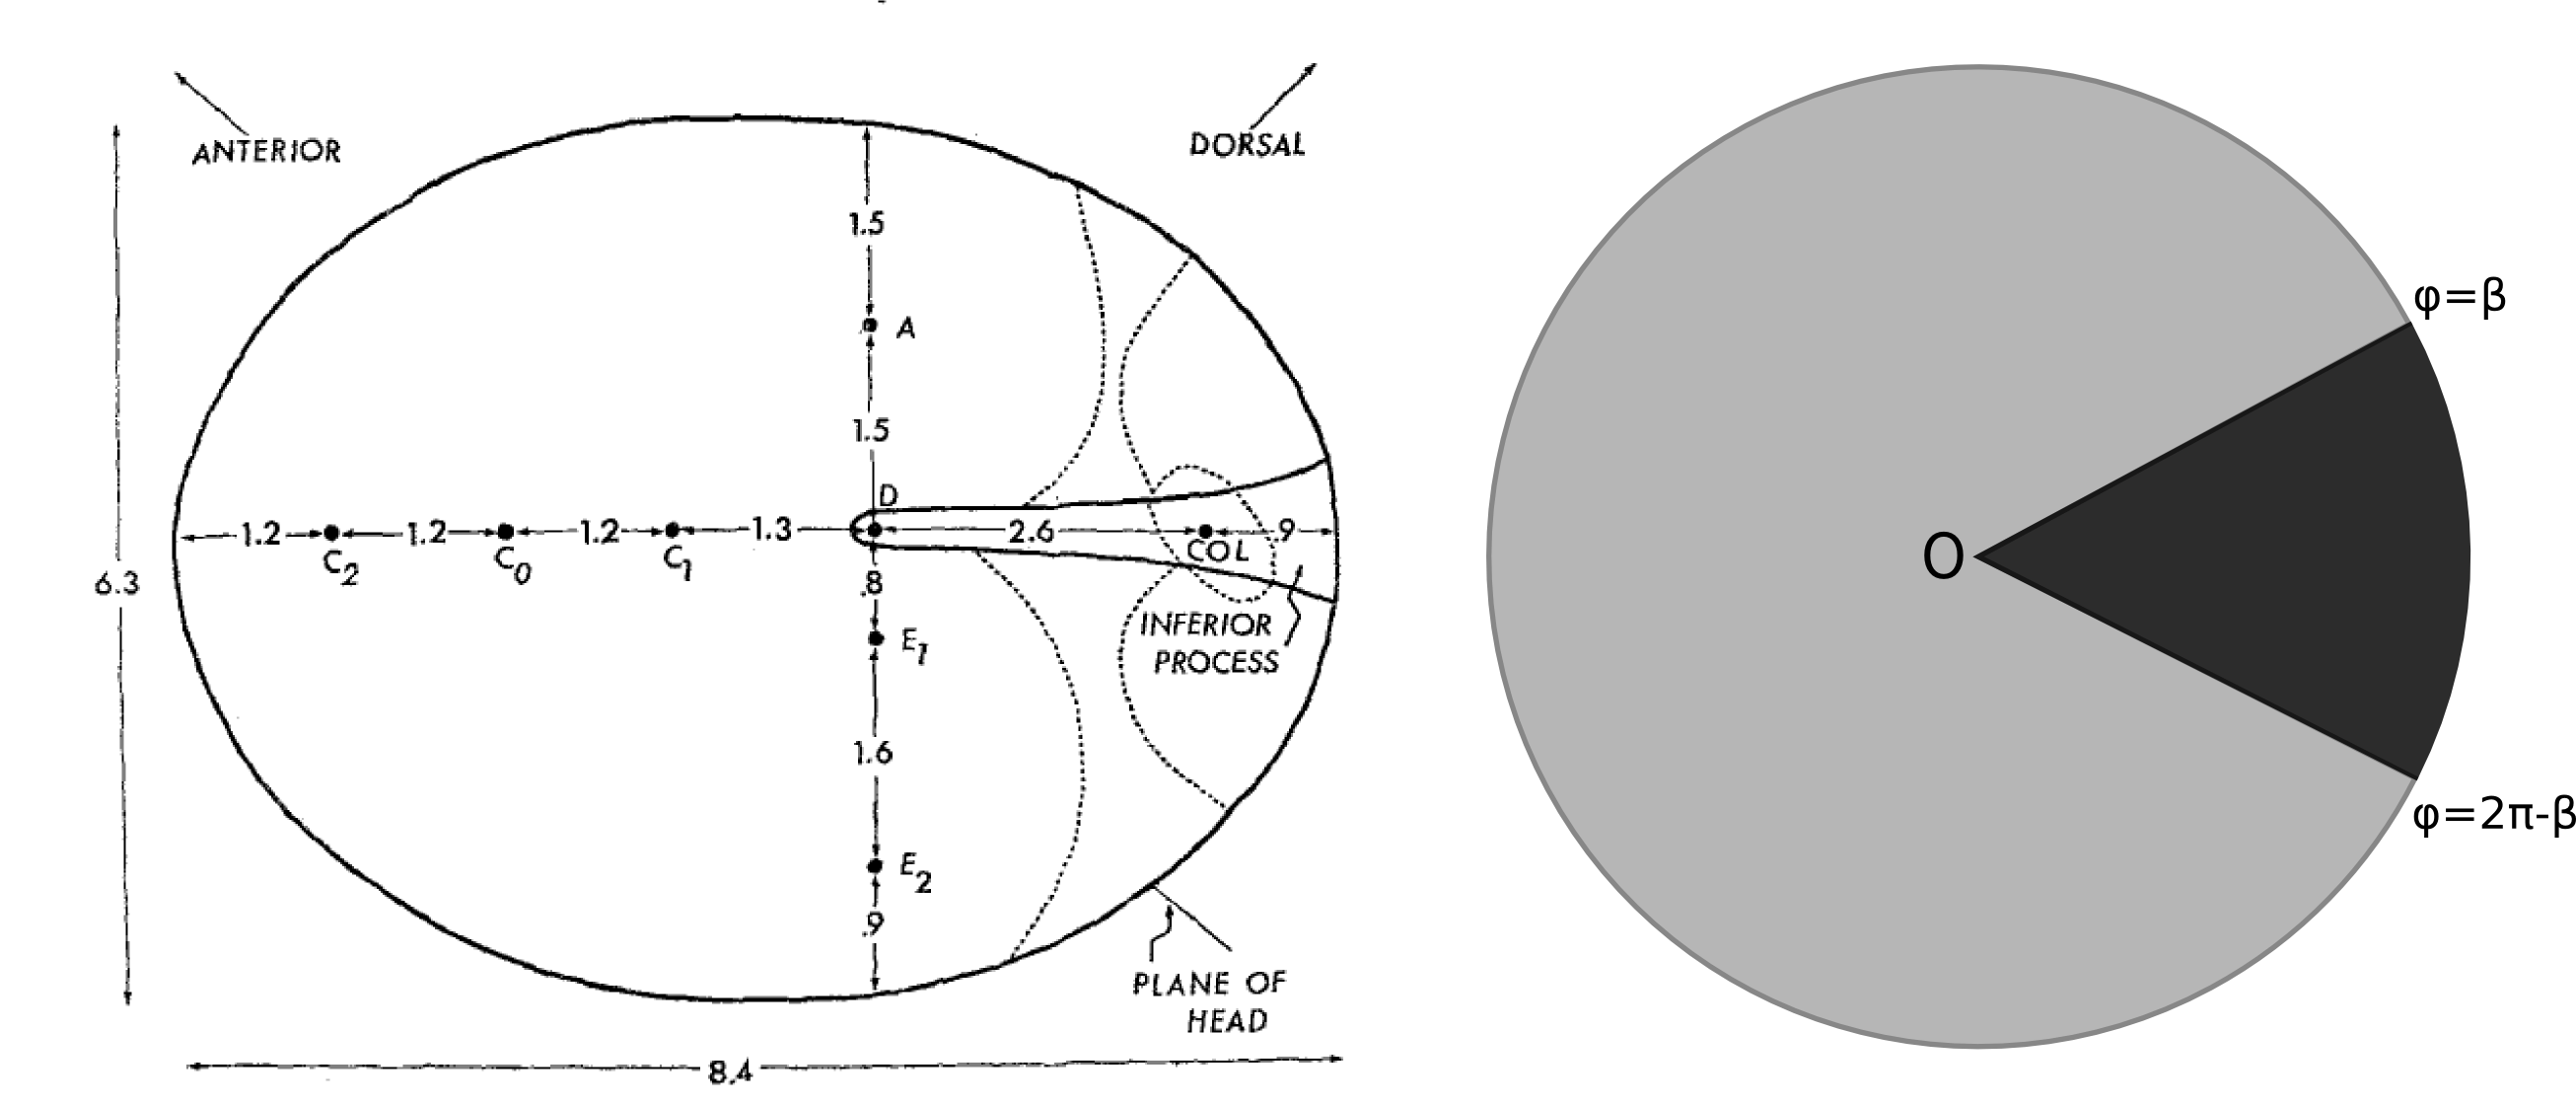
\includegraphics[width=.3\linewidth]{Diagrams/extracolumella2.png}
 \caption[Tympanic membrane model]{Model of the loaded tympanice membrane. The lightly shaded region is modelled as a linear elastic membrane whereas the darkly shaded region 
 ($\beta<\phi<2\pi-\beta$) represents the contact surface of the extracolumella and the membrane. $\beta$ is estimated from the anatomical data.}
\end{figure}
As a result of this, the tympanum cannot vibrate freely. For most frequencies, the extracolumella vibrates as a completely stiff
bar. Flection occurs at 
\subsection{Sound Input}

\section{Derivation of the Model}
We will now use the previously described physical model to derive the main quantities of interest in the ICE model. We first find an expression
for the pressure distribution in the cylindrical cavity and for the membrane vibrations subject to an external stimulus. We then apply the 
appropriate boundary conditions to relate the membrane vibrations to the internal pressure and find the expression for the membrane
vibrations as a function of direction and frequency.
\subsection{Internal Cavity}
We assume that the air inside the cavity obeys linear acoustics (briefly discussed in \ref{acousticappendix}). The pressure distribution inside the cavity
is therefore given by the $3$D acoustic wave-equation in cylindrical polar coordinates,	
\begin{equation}\label{pressurewaveeqn}
 \frac{1}{c^2}\frac{\partial^2 p(x,r,\phi,t)}{\partial t^2}=\frac{1}{r}\frac{\partial}{\partial r}\left(r\frac{\partial p(x,r,\phi,t)}{\partial r}\right)
 +\frac{1}{r^2}\frac{\partial p(x,r,\phi,t)}{\partial \phi^2}+\frac{\partial p(x,r,\phi,t)}{\partial x^2}
\end{equation}
where $c$ is the sound propagation velocity. The complete solution must take into account the boundary conditions at and within the cavity walls and the
ones at the air-membrane interface. We also note that the above equation implies that the animal's mouth is closed, which is typical for a waiting
animal. In order to solve \eqref{pressurewaveeqn} for a particular frequency $f$ (angular frequency $\omega=2\pi f$), we use the following
separation ansatz
\begin{equation}\label{pseparationansatz}
  p(x,r,\phi,t)=f(x)g(r)h(\phi)e^{j\omega t}
\end{equation}
which after substitution into the acoustic wave-equation leads to,
\begin{equation}\label{pseparationansatz2}
\begin{split}
 k^2f(x)g(r)h(\phi)+&f(x)h(\phi)\left[\frac{\partial^2 g(r)}{\partial r^2} + \frac{1}{r}\frac{\partial g(r)}{\partial r}\right] \\
 &+f(x)g(r)\frac{1}{r^2}\frac{\partial h(\phi)}{\partial \phi}+\frac{\partial^2 f(x)}{\partial x^2}=0
\end{split}
\end{equation}
with $k:=\omega/c$. This results in the following set of separated ODE's,
\begin{align}
 \frac{d^2 f(x)}{dx^2}+\zeta^2f(x)&=0\\
 \frac{d^2 h(\phi)}{d\phi^2}+q^2h(\phi	)&=0\\
 \frac{\partial^2 g(r)}{\partial r^2} + \frac{1}{r}\frac{\partial g(r)}{\partial r}+\left[(\displaystyle\underbrace{k^2-\zeta^2}_{=:\nu^2})-\frac{q^2}{r^2}\right]g(r)&=0\label{besselequation1}
\end{align}
with separation constants $q$ and $\zeta$. The last equation is the Bessel differential equation \cite[p.~313]{copsonbessel} and its general solution is given by,
\begin{equation}
 g(r)=C_{qs}J_q(\nu r)+D_{qs}Y_q(\nu r).
\end{equation}
$J_q$ and $Y_q$ are the order-$q$ Bessel functions of the first and second kind respectively. The Bessel function of the second kind can be ignored as it diverges at $r=0$.
The solutions to the separated equations are therefore given by,
\begin{equation}
 f(x)=e^{\pm \zeta x},\ h(\phi)=e^{\pm j\phi},\text{and}\ g(r)=J_q(\nu r)
\end{equation}
with a specific solution to \eqref{pressurewaveeqn} given by,
\begin{equation}\label{specificpressure1}
 p(x,r,\phi;t)=\left[(A^+e^{jq\phi}+A^-e^{-jq\phi})e^{j\zeta x}+(B^+e^{jq\phi}+B^-e^{-jq\phi})e^{-j\zeta x}\right]J_q(\nu r)e^{j\omega t}.
\end{equation}
The coefficients $A^\pm$, $B^\pm$, $q$, $\zeta$ and $\nu$ will be subsequently determined by the boundary conditions. 

In general, the time component of the pressure also has a \textit{backward-moving} component, i.e. $e^{-j\omega t}$. By making the ansatz in \eqref{pseparationansatz}, 
we have implicitly made use of the fact that the form of the input constrains the pressure to only have a \textit{forward-moving} component, i.e. $e^{j\omega t}$.  
\subsubsection{Pressure Boundary Conditions}
There are three sets of boundary conditions - 
\begin{itemize}
 \item Continuity and smoothness in $\phi$ which is equivalent to $h(0)=h(2\pi)$ and $h^\prime(0)=h^\prime(2\pi)$ where, $h^\prime=dh/d\phi$.
 \item Vanishing of the normal derivative at the cavity walls - $g^\prime(a_C)=0$ ($a_C$ is the radius of the cylinder).
 \item Equating the membrane velocity to the air velocity at the membrane boundaries (to be discussed in the next section).
\end{itemize}
The first set of requirements is obvious. This reduces \eqref{specificpressure1} to 
\begin{equation}\label{specificpressure2}
 p(x,r,\phi;t)=\left[Ae^{j\zeta x}+Be^{-j\zeta x}\right]\cos q\phi J_q(\nu r)e^{j\omega t}.
\end{equation}
With $q$ constrained to be an integer.

The second and third are a result of the so called ``no-penetration'' boundary-condition
of fluid-mechanics. It arises from the from the fact that the cavity wall is an impermeable boundary. This translates 
into the requirement that the normal fluid-particle velocity should vanish (\cite[p.~111]{pozrikidisFluid}).
The fluid-particle velocity ($\mathbf{v}$) is related to the pressure by, 
\begin{equation}\label{pressurevelocityrelation}
 -\rho\frac{\partial \mathbf{v}}{\partial t}=\nabla p
\end{equation}
At the cylindrical cavity wall, the normal velocity is in the radial direction.
Substituting the expression for pressure in \eqref{specificpressure1} in the above equation leads to
a Neumann boundary condition for the pressure,
\begin{align}\label{radialnopenetration}
 v_r=-\left.\frac{1}{j\rho\omega}\frac{\partial p(x,r,\phi;t)}{\partial r}\right\vert_{r=a_C}&=0\nonumber\\
    \Rightarrow\left.\frac{\partial J_q (\nu r)}{\partial r}\right\vert_{r=a_C}&=0
\end{align}
This constrains $\nu$ to a discrete set of values which correspond to the local minima and maxima
of $J_q$. We can therefore index $\nu$ by $q$ and $s=0,1,2,3,\ldots$ with $\nu_{qs}=z_{qs}/a_C$:
$z_{qs}$ being the $s^{th}$ extremum of the order-$q$ Bessel function of the first kind.
This results in a discrete set of modes that satisfy \eqref{pressurewaveeqn} which are given
by,
\begin{equation}\label{specificpressure3}
 p_{qs}(x,r,\phi;t)=\left[A_{qs}e^{j\zeta_{qs}x}+B_q{s}e^{-j\zeta_{qs}x}\right]f_{qs}(r,\phi)e^{j\omega t}
\end{equation}
where we have added the subscripts $q$ and $s$ to $\zeta$ and denoted the $(r,\phi)$ part of \eqref{specificpressure2}
by $f_{qs}(r,\phi)$. Effectively, the
modes are 3D waves propagating with wave numbers $\zeta_{qs}$ in the $x$-direction and $\nu_{qs}$ in the radial
direction. The first of these modes (corresponding to $q=0,s=0$) is of particular importance. Since the first
maximum of $J_0$ occurs at $r=0$, we have $\nu_{00}=0$. This leads to the first mode being a plane-wave which
is constant in $r$ and $\phi$ and only varies in $x$. 

A very useful property of the above modes is their orthgonality, i.e.
\begin{equation}\label{pressureorthogonality}
 \int_\Omega dVp_{q_1s_1}p_{q_2s_2}=0,\ if\ q_1\neq q_2\ or\ s_1\neq s_2
\end{equation}
the integral is over the volume of the cylinder. This is a consequence of the fact that for different $q$'s
the cosine parts of the modes are orthogonal whereas for a given $q$ the Bessel parts are orthogonal for
different $s$'s or expressed as an equation,
\begin{equation}\label{besselorthogonality}
 \int dS f_{q_1s_1}f_{q_2s_2}=0,\ q_1\neq q_2\ or\ s_1\neq s_2
\end{equation}
where $dS=rdrd\phi$ and the integral being taken over the disk of radius $a_C$.
We can therefore write the general solution to \eqref{pressurewaveeqn} as a linear combination of the orthogonal modes given in \eqref{specificpressure3},
\begin{equation}\label{pressuregeneral1}
 p(x,r,\phi;t)=\displaystyle\sum^\infty_{q=0}\displaystyle\sum^\infty_{s=0}\left(A_{qs}e^{j\zeta_{qs}x}+B_{qs}e^{-j\zeta_{qs}x}\right)f_{qs}(r,\phi)e^{j\omega t}
\end{equation}
The remaining coefficients, $A_{qs}$ and $B_{qs}$, will be determined by equating the fluid-particle velocity to
the membrane velocity at both ends of the cylinder. To do so, we will first need to find an expression
for the membrane vibrations and subsequently make use of some simplifying approximations.

\subsection{Vibration of the Membrane}
As a preliminary exercise, we will first derive expressions for the free and force-driven
vibrations of a circular membrane. We will then use our results to move on to the sectoral membrane 
which corresponds to the tympanum loaded by the extracolumella. Thi corresponds to the approximating
the extracolumella to have infinite mass. 
\subsubsection{Circular Membrane}
The equation of motion for the vibration of a rigidly clamped circular membrane of radius $a_M$ solves for the membrane displacement $u$ at
a point $(r,\phi)$ with $r<a$ and $0<\phi<2\pi$. It is given by,
\begin{equation}\label{membraneequation1}
 \begin{split}
 -\frac{\partial^2 u(r,\phi;t)}{\partial t^2}-2\alpha\frac{\partial u(r,\phi;t)}{\partial t}+c^2_M \left[\frac{1}{r}\frac{\partial}{\partial r}\left(r\frac{\partial u(r,\phi,t)}{\partial r}\right)\right. +\frac{1}{r^2}&\left.\frac{\partial u(r,\phi,t)}{\partial \phi^2}\right]
 \\ &=\frac{1}{\rho_M d}\Psi(r,\phi;t)
 \end{split}
\end{equation}
subject to the boundary condition $u(r,\phi;t)|_{r=a_M}=0$.. We've defined the following membrane material properties,
\begin{itemize}
 \item $c_M$ - propagation speed of vibrations.
 \item $\alpha (>0)$ - the damping coefficient.
 \item $\rho_M$ - density.
 \item $d$ - thickness.
\end{itemize}
$\Psi(r,\phi;t)$ is the pressure on the membrane surface at $(r,\phi)$. In our discussion we are only concerned with periodic and uniform 
pressure acting on the membrane surface. This is justified by the fact that for typical hearing ranges of these animals, the wavelength
of sound is much greater than the membrane size and any spatial variation can be neglected.
\subsubsection*{Free Vibrations}
\noindent\textbf{Undamped Membrane}: We first determine the eigenmodes of an undamped circular membrane by solving \eqref{membraneequation1} for $\alpha=0,\ \Psi=0$. To do this 
we make a separation ansatz just as we did in \eqref{pseparationansatz},
\begin{equation}\label{mseparationansatz}
 u(r,\phi;t)=f(r)g(\phi)h(t)
\end{equation}
This gives us the following set of equations
\begin{align}
 \frac{\partial^2 f(r)}{\partial r^2} + \frac{1}{r}\frac{\partial f(r)}{\partial r}+\left[\mu^2-\frac{m^2}{r^2}\right]f(r)&=0\label{besselequation2}\\
  \frac{d^2 g(\phi)}{d\phi^2}+m^2g(\phi)&=0\\
 \frac{d^2 h(t)}{dt^2}+c^2_M\mu^2h(t)&=0
\end{align}
with separation constants $\mu$ and $m$. The solution of the first of these equations should already be familiar to us from the previous section - $J_m(\mu r)$,
 the order-$m$ Bessel function of the first kind. The boundary conditions in $\phi$ direction remain the same resulting in,
\begin{equation}\label{specificmembrane1}
 u(r,\phi;t)=\left[(M^+e^{jm\phi}+M^-e^{-jm\phi}\right)e^{jc_M\mu t}+(N^+e^{jm\phi}+N^-e^{-jm\phi})e^{-jc_M\mu t}] J_m(\mu r)
\end{equation}
Unlike in the case of the internal cavity, we require $u$ to vanish at the boundary so we have a Dirichlet boundary condition which
effectively requires: $J_m(\mu a_M)=0$. This constrains $\mu$ to a discrete set of values which correspond to the zeros of $J_m$. The eigenmodes of a 
the circular membrane are therefore given by,
\begin{equation}\label{membraneeigen}
\begin{split}
 u_{mn}(r,\phi;t)=\left[(M^+_{mn}e^{jm\phi}+M^-_{mn}e^{-jm\phi})\right.& e^{j\omega_{mn} t}+ \\
 &\left.(N^+_{mn}e^{jm\phi}+N^-_{mn}e^{-jm\phi})e^{-j\omega_{mn} t}\right] J_m(\mu_{mn} r)
 \end{split}
\end{equation}
where $\mu_{mn}=z_{mn}/a_M$, $z_{mn}$ being the $n^{th}$ zero of $J_m$ and, $\omega_{mn}=c_M\mu_{mn}$ is
the eigenfrequency of the $(m,n)$ eigenmode. At this point $m$ can take any positive real value -- a fact that will
help us solve the sectoral membrane problem. However, in the case of a full circular membrane -- as in the case
of the pressure inside a cylindrical cavity -- requirements of continuity and smoothness in $\phi$ reduce \eqref{membraneeigen}
to,
\begin{equation}\label{circularmembraneeigen}
 u_{mn}(r,\phi;t)=\cos m\phi J_m(\mu_{mn} r)\left[M_{mn}e^{j\omega_{mn} t}+N_{mn}e^{-j\omega_{mn} t}\right]
\end{equation}
with $m=0,1,2,\ldots$ with the $(m,n)$ eigenmodes forming an orthogonal set. For later convenience we denote the spatial
part of the above mode by $u_{mn}(r,\phi)$. We note that unlike in the case of the internal cavity, the free membrane has components
that are both forward- and backward-moving in time. The presence of a driving force, however, will simplify the expressions.

\vspace{\baselineskip}
\noindent\textbf{Damped Membrane}: For a damped membrane, i.e. $\alpha\neq 0$, the spatial part of the above eigenmodes remains the same. The form of the
time-dependent part is given by the solution of the equation,
\begin{equation}\label{dampedtimepart}
 \frac{d^2 h_{mn}(t)}{dt^2}+2\alpha \frac{d h_{mn}(t)}{dt}+\omega_{mn}^2h_{mn}(t)=0.
\end{equation}
Assuming $h_{mn}$ takes the form $e^{j\widetilde{\omega}_{mn}}$ leads to a quadratic equation with solutions,
\begin{align}
 \widetilde{\omega}_{mn}&=j\alpha\pm\omega_{mn}^*\\
 \omega_{mn}^*&=\sqrt{\alpha^2+\omega^2_{mn}}
\end{align}
We require the membrane displacement to remain finite as $t\rightarrow\infty$. We can therefore neglect the $e^{-j\widetilde{\omega}_{mn}}$ terms leading
to,
\begin{equation}\label{circularmembranedampedeigen}
 \widetilde{u}_{mn}(r,\phi;t)=\cos m\phi J_m(\mu_{mn} r)\left[M_{mn}e^{j\omega_{mn}^* t}+N_{mn}e^{-j\omega_{mn}^* t}\right]e^{-\alpha t}
\end{equation}
The general solution is given by a linear combination of the above and the coefficients are determined by initial conditions -- for example,
membrane displacement and velocity at $t=0$.
\subsubsection*{Forced Vibrations}
For a periodically driven membrane, there are two components of the full solution for forced vibrations. The first of these is the steady state solution which
oscillates with the same frequency as the input and does not depend on the initial conditions - $u_{ss}$. The second of these is the transient solution that depends
on the initial conditions but not on the driving pressure - $u_t$. 

\noindent\textbf{Steady State Solution}: The steady state solution is expressed as a linear combination of the spatial part
of the above eigenmodes and is given by,
\begin{equation}\label{membraness1}
 u_{ss}(r,\phi ;t)=\displaystyle\sum^\infty_{m=0}\sum^\infty_{n=1} C_{mn}\cos m\phi J_m(\mu_{mn} r)e^{j\omega t}.
\end{equation}
Substituting this expression in \eqref{membraneequation1} with $\Psi=pe^{j\omega t}$ gives,
\begin{align}
 &\displaystyle\sum^\infty_{m=0}\sum^\infty_{n=1} \Omega_{mn}C_{mn}\cos m\phi J_m(\mu_{mn} r)e^{j\omega t}=pe^{j\omega t}\label{membraness2}\\
 &\text{where,  }\Omega_{mn}=\rho_M d (\omega^2-2j\alpha\omega-\omega^2_mn)\label{omegafirstdef}.
\end{align}
Using the orthogonality of the eigenmodes, the coefficients $C_{mn}$ can be calculated,
\begin{equation}\label{sscoeffs}
 C_{mn}=\frac{p\int dS u_{mn}}{\Omega_{mn}\int dS u^2_{mn}}
\end{equation}
with the integral this time being taken over the circular disk of radius $a_M$.

\vspace{\baselineskip}
\noindent\textbf{Transient Solution}: The transient solution is effectively a solution of the free damped membrane, i.e. a linear 
combination of the eigenmodes given in \eqref{circularmembranedampedeigen}. Therefore,
\begin{equation}\label{membranet1}
 u_t(r,\phi;t)=\displaystyle\sum^\infty_{m=0}\sum^\infty_{n=1}\cos m\phi J_m(\mu_{mn} r)\left[M_{mn}e^{j\omega_{mn}^* t}+N_{mn}e^{-j\omega_{mn}^* t}\right]e^{-\alpha t}.
\end{equation}
The complete solution is given by $u=u_t+u_{ss}$ and the coefficients $M_{mn}$ and $N_{mn}$ are determined by the initial conditions (at $t=0$).

\vspace{\baselineskip}
\textbf{Steady State Approximation}: The damping coefficient $\alpha$ is usually given in terms of the membrane fundamental frequency and a quality factor $Q$ as $\alpha=\omega_{01}/2Q$. For the tympani
we will be concerned with, $\alpha\sim 4000s^{-1} $ for the larger lizards and $\alpha\sim 8000s^{-1}$ for the smaller ones. Therefore, the transient response can be 
safely neglected for their hearing ranges.
\subsubsection{Sectoral Membrane}
The eigenmodes of the sectoral membrane proceeds from \eqref{membraneeigen} onwards. We now have a new set of boundary conditions in $\phi$.
The extracolumella is modelled as a triangular plate of infinite mass which constrains the membrane displacement to go to zero at $phi=\beta$
and $\phi=2\pi-\beta$. This results in the following set of eigenmodes,
\begin{equation}\label{sectoraleigenmode}
 u_{mn}(r,\phi;t)=\sin \kappa(\phi-\beta) J_\kappa(\mu_{mn} r)\left[M_{mn}e^{j\omega_{mn} t}+N_{mn}e^{-j\omega_{mn} t}\right]
\end{equation}
where $\kappa[m]=\frac{m\pi}{2(\pi-\beta)}$, $m=1,2,3,\ldots$. We see that the $r$ part of the above mode is given by the
order-$\kappa$ Bessel function of the first kind; $\mu_{mn}$ being its $n^{th}$ zero, as before. The solution for the damped
membrane follows in an identical way.
It is apparent from the form of the above modes that, unlike in the case of the circular membrane eigenmodes, these modes
are no longer circularly symmetric. We plot the first few of these modes in increasing order of frequency.